% !TEX encoding = UTF-8
% !TEX TS-program = pdflatex
% !TEX root = ../Tesi.tex
% !TEX spellcheck = en-EN

%************************************************
\part{Introduction}
\label{par:introduction}
%************************************************

Particles in various forms - ranging from raw materials to food grains and pharmaceutical powders - 
play a major role in a variety of industries, including process industry and metallurgy. 
In his book, \citet{RefWorks:117} stated that "between 1 and 10\% of all the energy is used in 
comminution, i.e. the processes of crushing, grinding, milling, micronising". 

can not be easily characterized as for instance a steel beam. 

Fig. \ref{fig:050steel} \\

\begin{figure}[!htb]
\centering
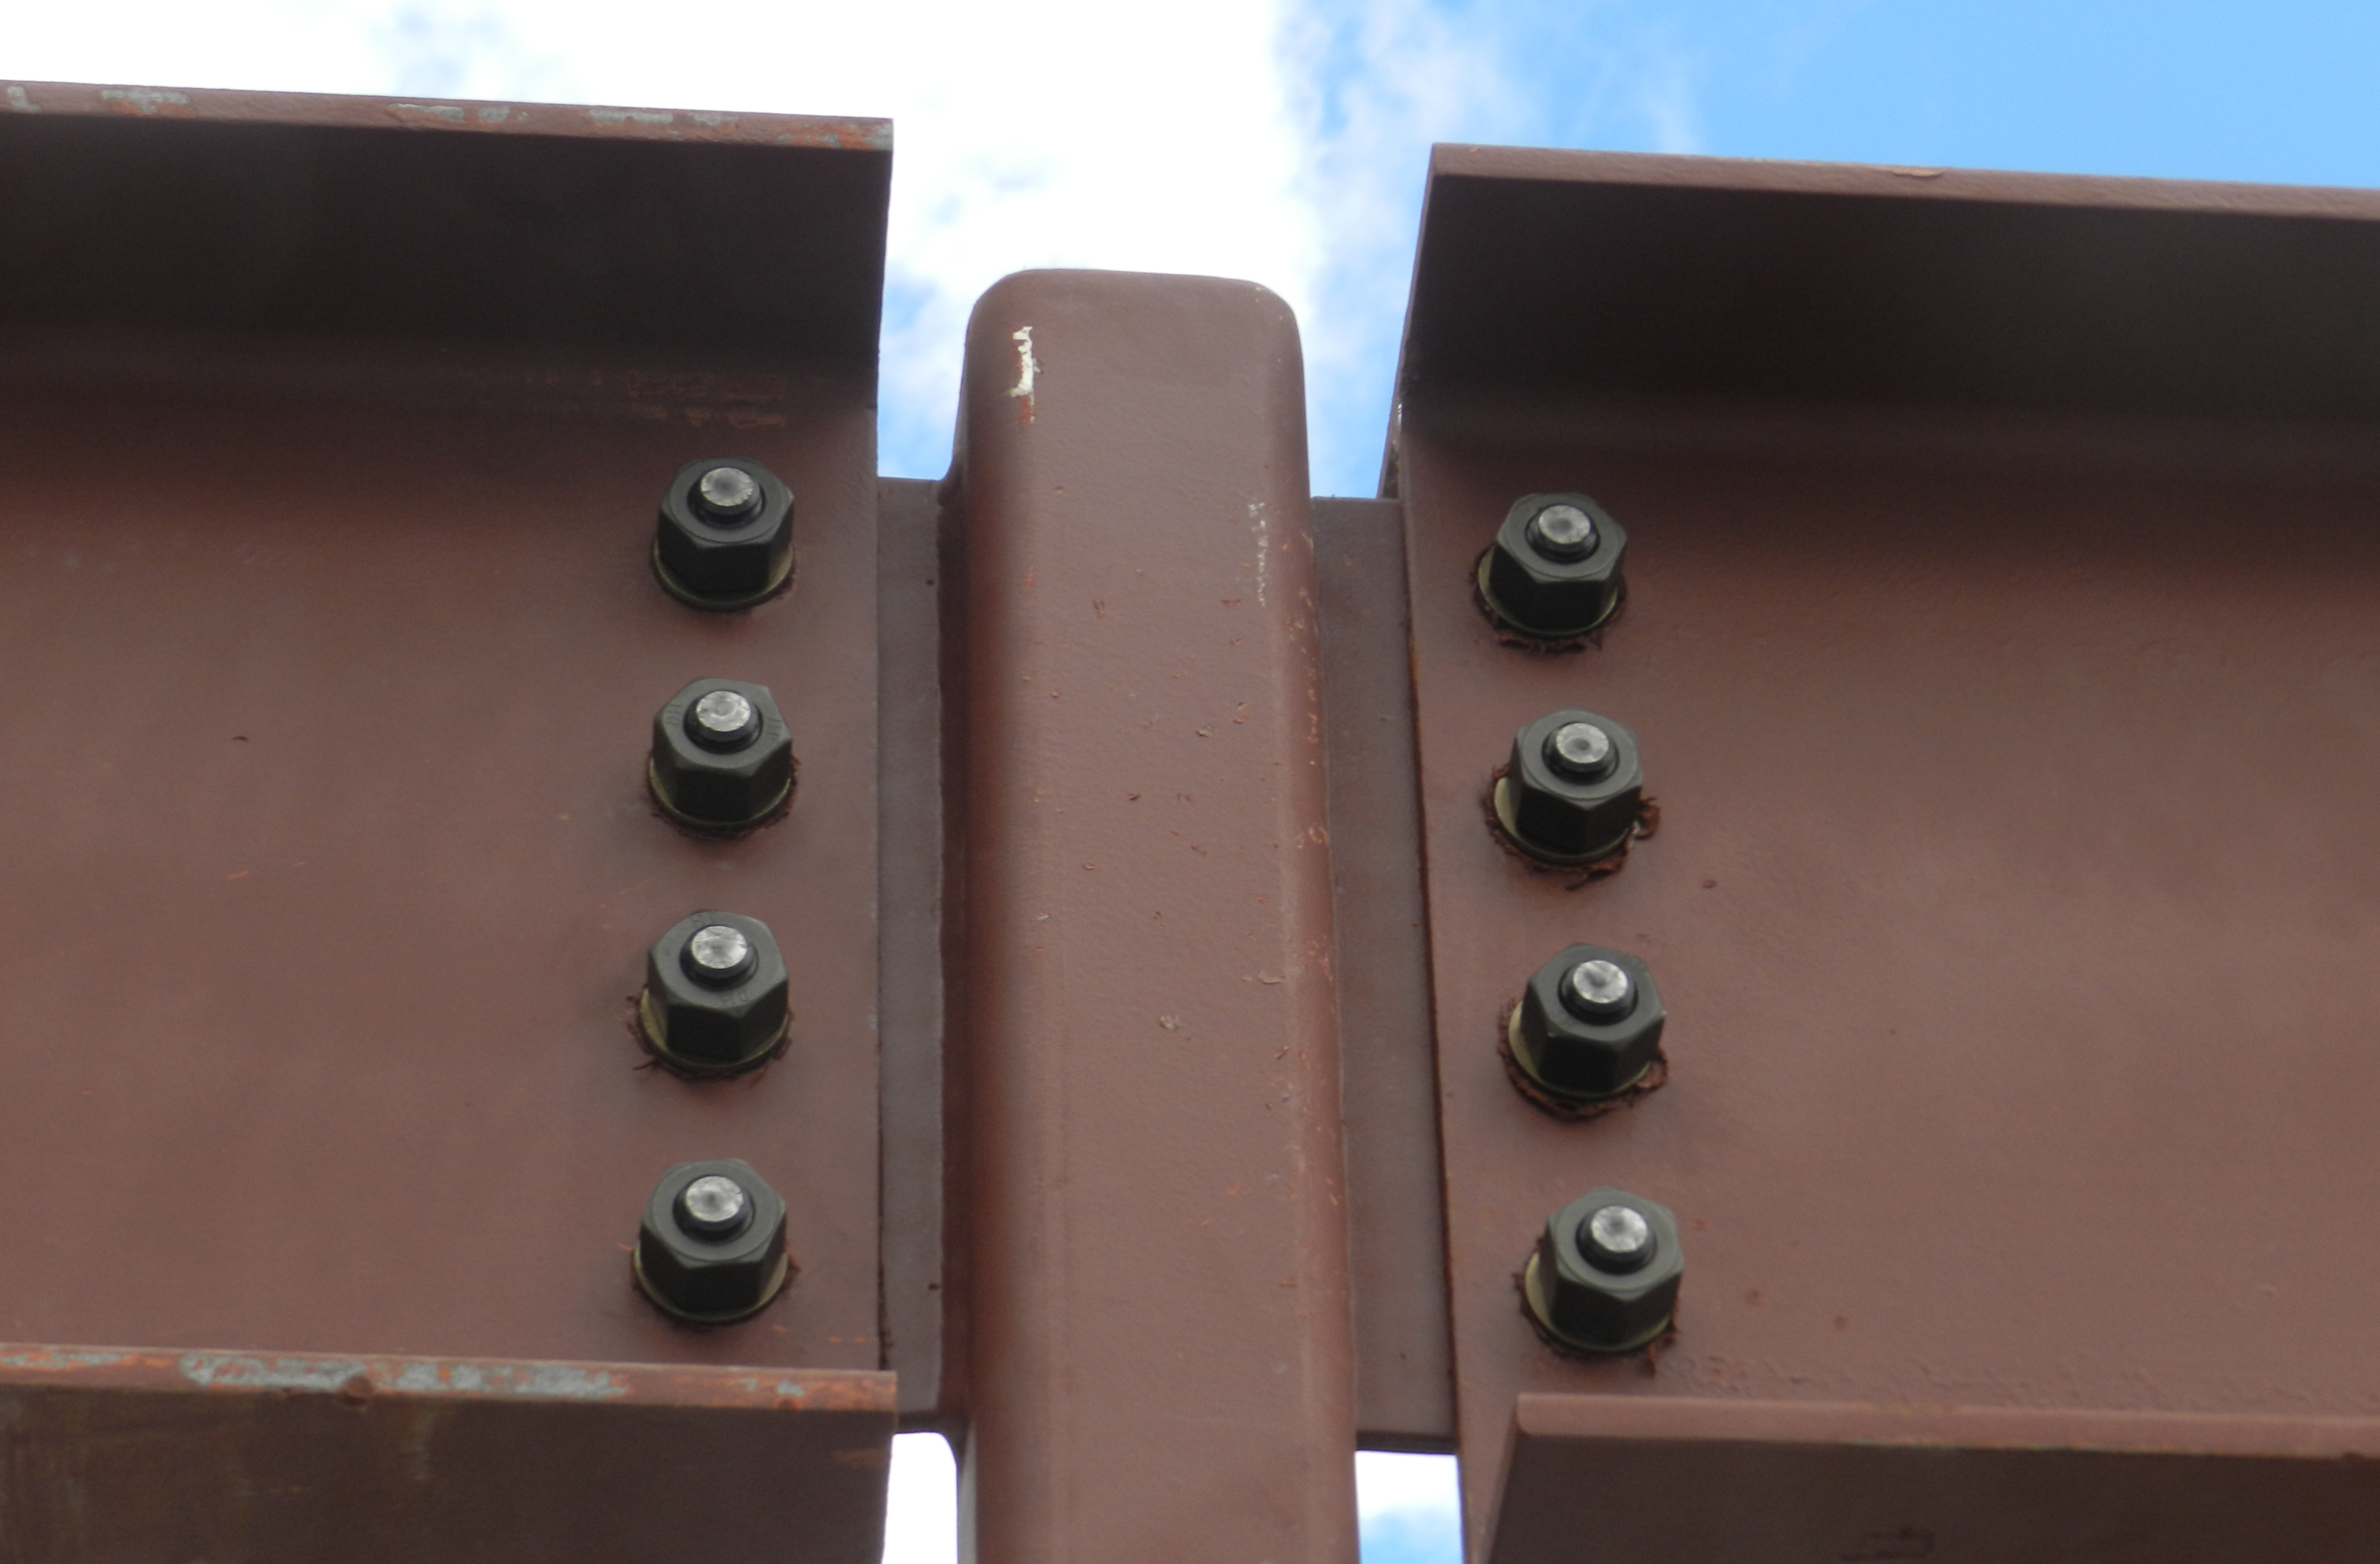
\includegraphics[width=.50\columnwidth]{images/050steel}
\caption[Steel]{Steel.}
\label{fig:050steel}
\end{figure}

Fig. \ref{fig:054bsgmaterials} \\
\begin{figure}[!htb]
\centering
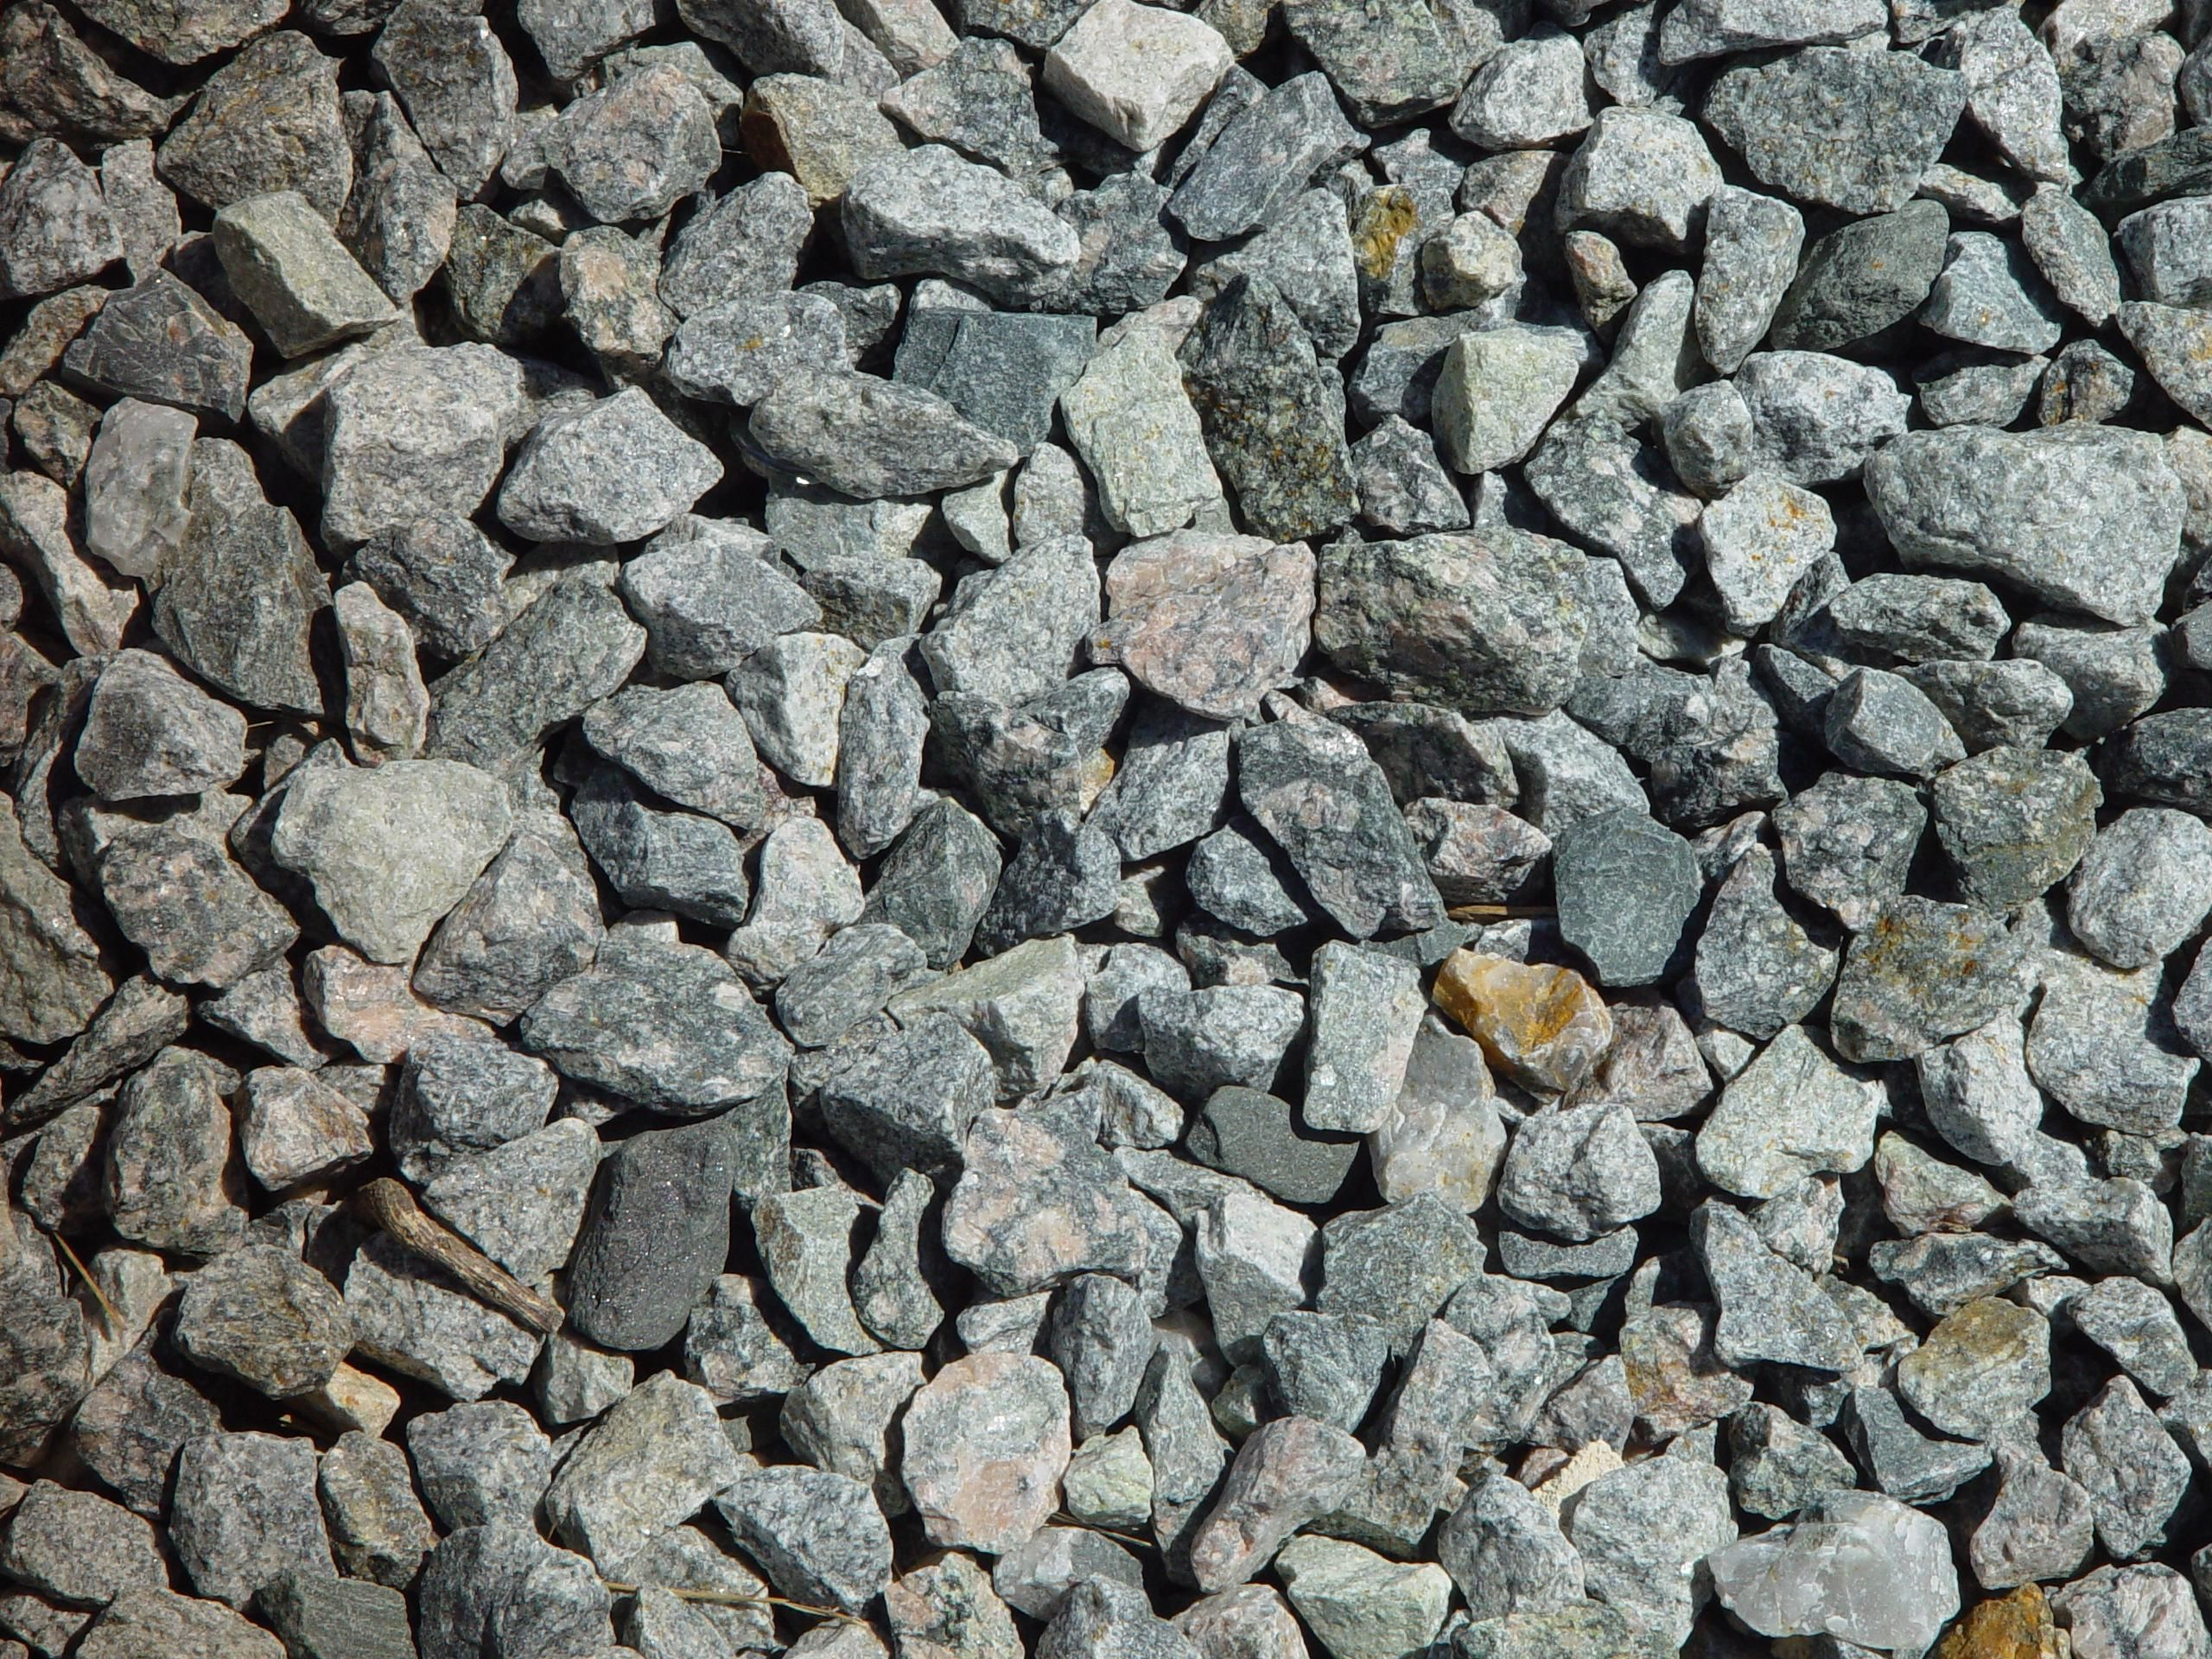
\includegraphics[width=.50\columnwidth]{images/133gravel}
\caption[Gravel]{Gravel.}
\label{fig:133gravel}
\end{figure}

Discrete Element Methods ($DEMs$) , "a special class of numerical schemes for
simulating the behavior of discrete, interacting bodies", are widely used to 
simulate particle behaviour in these granular processes
(\citet{RefWorks:130}).\\
A set of experimental and numerical solutions, together with artificial neural networks, can improve the accuracy 
and the range of applicability of the characterization of particles properties, and reduce the computational costs.
After the data collection (thanks to a set of characterization devices) physical key parameters 
(bulk-macro behavior) of particles are identified.
Meanwhile, combinations of DEM-microscopic parameters have been simulated, each leading to a different 
numerical bulk-macroscopic behavior, through DEM (LIGGGHTS) and CFDEM (CFDEMcoupling). 
The predictive capability of any simulation strongly depends on the validity of the particle based 
simulation parameters. To ensure it is not necessary to evaluate a huge number of parameter sets, 
but rather to evaluate the
sensitivity of the bulk behavior with respect to individual particle based parameters. 
This can be realized efficiently by Artificial Neural Networks. 
Inside the NN neurons are linked to particle based input parameters. 
By matching the output of the artificial neural network to DEM simulation results the network is 
trained (i.e. individual neurons are weighted), with excellent regression results. 
Later, the trained neural network can be used to predict additional valid sets of particle based 
simulation parameters: we compare the macro-bulk behavior of these sets against the experimental 
data collected, gaining averages and validity range. 
In fact, we obtain valuable information about the dependence of bulk solid behavior on individual 
particle properties and eventually mutual dependencies.

Fig. \ref{fig:048neuron0}
\begin{figure}[!htb]
\centering
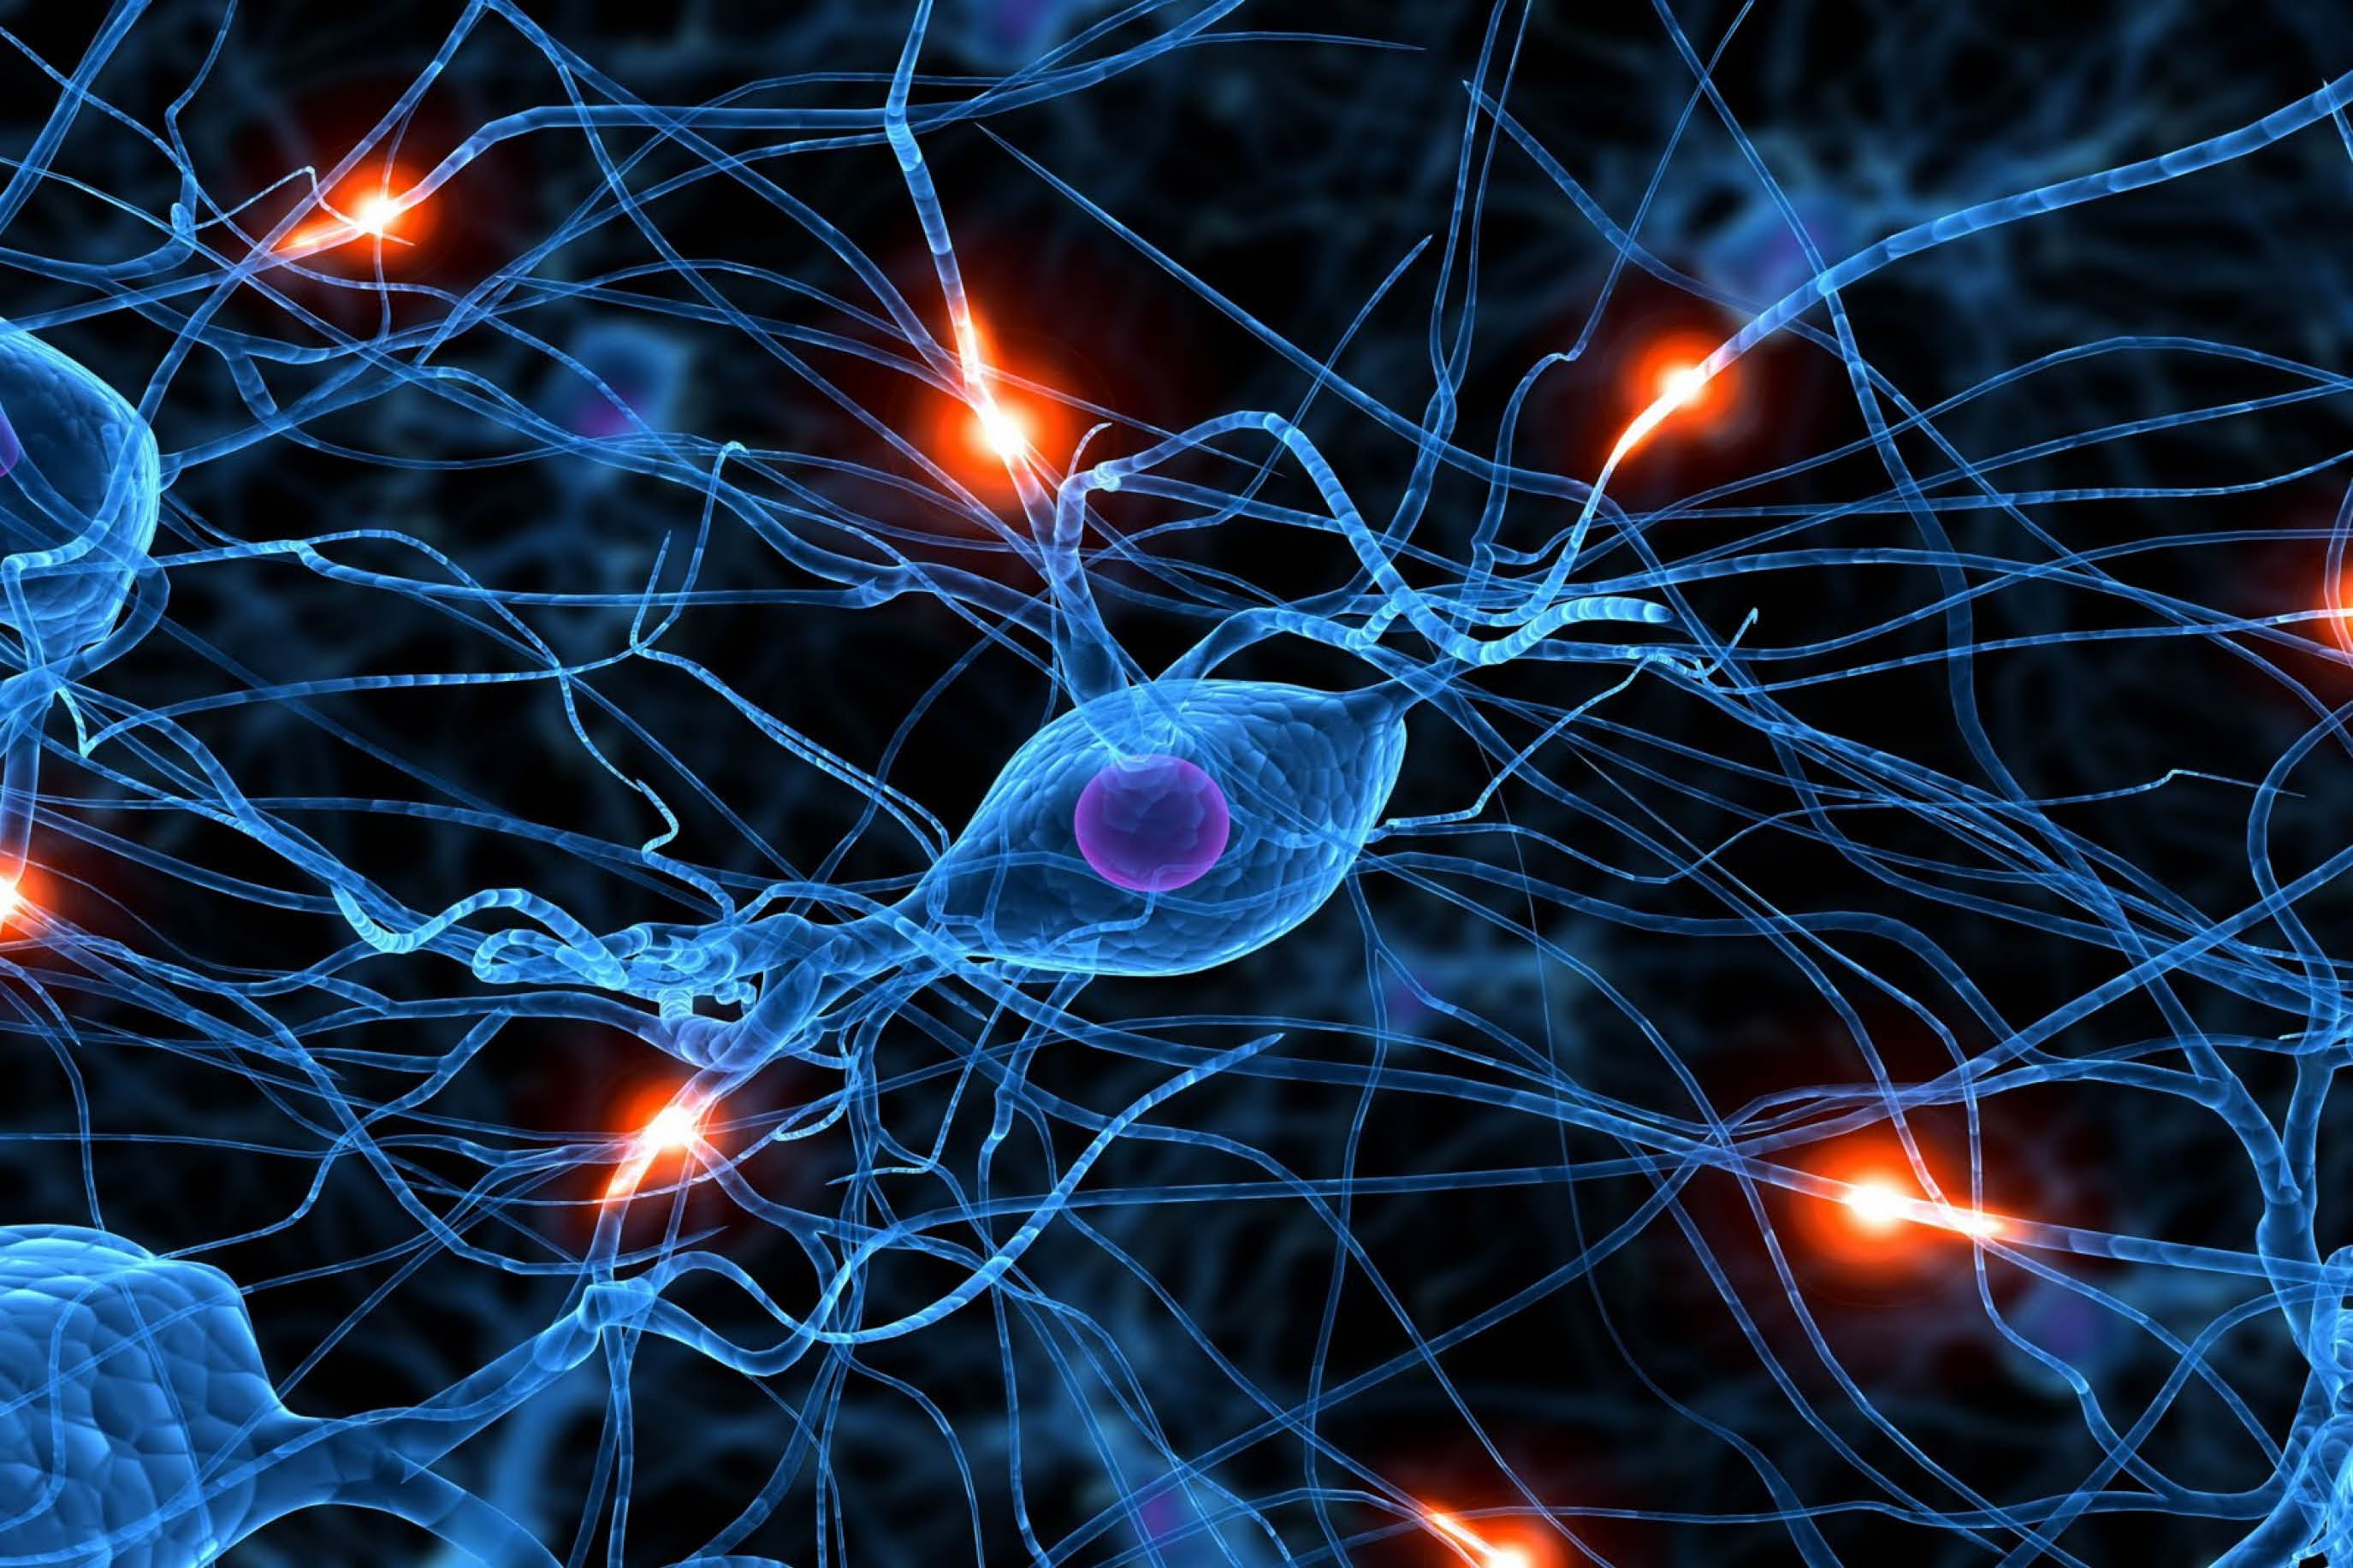
\includegraphics[width=.50\columnwidth]{images/048neuron0}
\caption[Biological inspiration]{Biological inspiration for the Artificial
Neural Networks: a human neuron with the incoming electric signals
\cite{RefWorks:158}.}
\label{fig:048neuron0}
\end{figure}

We could start with an example of piled particles, more specifically called the
drained angle of repose. This angle of repose, characteristic of the bulk
macroscopic behaviour of the ensemble, is originated from the microscopic
characteristics of each particle.
At the same time $DEM$ have been widely used to picture this behaviour, but the
not negligible computational time have been always a major setback of these
efforts.
An efficient hardware implementation of this algorithm for fast particle
characterization is still investigated.

In fact, gravels, or granular particles in general, are far from being a well-defined material, for instance a steel beam
For continuous materials (e.g. steel) simulation parameters are readily available.
In case of a pile of particles the sum of discrete particle properties determines the pile's macroscopic behavior 
(e.g. angle of repose).
In discrete particle simulations particle based parameters (e.g. contact parameters) determine the macroscopic behavior 
of the ensemble.
Unfortunately, particles are not uniform and particle based simulation
parameters are difficult to obtain, and also depends on the numerical shape
(polyhedral, multi-spheres, and simple spheres).
Discrete Element Method requires parameters for the individual contact, but characterize every particle is prohibitive;
We need to find average contact parameters that lead to the expected bulk effect;
Measurement of a BULK parameter value, through calibration we obtain the
individual contact parameters:
\begin{enumerate}
\item{Chose initial set of parameters}
\item{DEM simulation}
\item{Compare macroscopic DEM simulation results with experiments}
\item{Choose new parameters}
\end{enumerate}

By our calibration procedure we obtain valid sets of particle based simulation parameters.
Ok, but that's very time consuming, because in each control loop we have to perform a complete DEM simulation
in our case we would need 9.900 days on a 32 core machine
It is not necessary to evaluate a huge number of parameter sets, rather we should try to evaluate the sensitivity 
of the macroscopic bulk behavior with respect to individual particle based parameters.
This can be realized efficiently by artificial neural networks!
In this artificial neural network neurons are linked to particle based input parameters. 
By matching the output of the artificial neural network to DEM simulation results the network is trained (i.e. individual neurons are weighted).
Later, the trained neural network can be used to predict additional valid sets of particle based simulation parameters. 

\begin{enumerate}
\item{Train neural network by 500 dedicated DEM simulations (time consuming)}
\item{Test another 6.250.000 combinations by the neural network (very fast)}
\item{Check if predictions of neural network are correct (by comparing with experimental  values)}
\end{enumerate}
Typically, less than 1\% of the tested parameter sets lead to correct
macroscopic results (i.e. 6.000 to 60.000 valid parameter sets).

By this assessment of particle based simulation parameters we obtain valuable information about the dependence of bulk solid behavior on individual particle properties.
First we can determine the validity range, mean and variance band of each input parameter
Next we can determine a probability density function for each input parameter
Then, we can investigate mutual dependencies
This calibration procedure is universal in a sense that the same artificial neural network can be harnessed for different macroscopic bulk behaviors.
Ok, that�s nice - but is this effort really necessary?
Yes, because the predictive capability of any DEM simulation strongly depends on the validity of the particle based simulation parameters! 
Finally, we can identify the final parameters!

\improvement{add some words on the applications}
